\documentclass{article}
\addtolength{\oddsidemargin}{-0.5in}
\addtolength{\evensidemargin}{-0.5in}
\addtolength{\topmargin}{-0.5in}
\addtolength{\textwidth}{+1.0in}
\addtolength{\textheight}{+0.5in}

%\parindent0cm
%\parskip.2cm
%\voffset0cm
%\hoffset0cm
%%%
%\oddsidemargin0cm
%\evensidemargin0cm
%\topmargin0cm
%\textwidth16.cm
%\textheight22cm

\usepackage{amsfonts,amsmath,amssymb}

\usepackage{diagbox}

% bold & italic
\newcommand{\bfit}[1]{\textbf{\textit{ #1 }}}

% multiline commments
\newcommand{\comment}[1]{}

% parentheses (, )
\newcommand{\lp}{\left(}
\newcommand{\rp}{\right)}
% brackets [, ]
\newcommand{\lbk}{\left \lbrack}
\newcommand{\rbk}{\right \rbrack}
% braces {, }
\newcommand{\lbc}{\left \lbrace}
\newcommand{\rbc}{\right \rbrace}
% empty delimeters
\newcommand{\la}{\left.}
\newcommand{\ra}{\right.}

% numbering in "*"-math-environments
\newcommand{\tack}{\addtocounter{equation}{1} \tag{\theequation}}

% Landau-O
\newcommand{\order}[1]{\ensuremath{\mathcal{O} \! \left( #1 \right)}}

% bra & ket
\newcommand{\bra}{\left \langle}
\newcommand{\ket}{\right \rangle}
% vacuum expectation value
\newcommand{\vev}[1]{\bra 0 \left| \, #1 \, \right| 0 \ket}

% MS-bar
\newcommand{\MSbar}{\ensuremath{{\overline{\textrm{MS}}}}}
% "correct" \epsilon, \varepsilon
\newcommand{\ep}{\ensuremath{\epsilon}}
% GeV
\newcommand{\GeV}{\ensuremath{\, \textrm{GeV}}}


\newcommand{\FORM}[0]{{\tt FORM}\ }

\usepackage{graphicx}
\graphicspath{{./figs/}}

\title{
  {\tt TopoID} -- \\
  a {\tt Mathematica} package for\\
  Topology Identification
}

\author{Jens Hoff}

% \date{}



\begin{document}



\maketitle

\begin{center}
\begin{verbatim}

              _______                      _   ____
 --->---+--- |__   __| ------------------ | | |  _ \  ---+--->---
         \      | |   __    ____     __   | | | | \ \    |
          +     | |  /  \  |  _ \   /  \  | | | |  \ \   |
          |\    | | / /\ \ | | \ \ / /\ \ | | | |  / /   +--->---
          | \   | | \ \/ / | |_/ / \ \/ / | | | |_/ /   /
          |  \  |_|  \__/  |  __/   \__/  |_| |____/   +
          |   \            | |                        / \
 --->-----+----+---------- |_| ----------------------+---+--->---


\end{verbatim}
\end{center}



\item Scale-less-ness:
  Rescale (some) loop-momenta like
  \begin{align}
    q_k \to q_k^\prime = \alpha_k q_k \quad \text{with} \quad k \in \{
    1, \ldots, n_{\rm int.} \}, \\
    I^\prime(\{ a_i \}) = f({\alpha_k}) I(\{ a_i \}) = I(\{ a_i \})
    \quad \Rightarrow \quad I(\{ a_i \}) = 0.
  \end{align}

\item Whenever a sub-topology (that is a certain set of factors is
  completely absent) is scale-less, the corresponding sub-topologies
  where additional factors appear purely as numerators are vanishing
  too:
  \begin{align}
    I(\{ a_i \}) = 0 \quad \text{with} \quad i \in s: a_i < 0, i \notin
    s: a_i = 0, \\
    \Rightarrow I^\prime(\{ a_i \}) = 0 \quad \text{with} \quad i \in s:
    a_i < 0, i \notin s: a_i \ge 0.
  \end{align}
  This can be explained as follows.  An additional numerator can always
  be separated into its terms which contain either constants (masses,
  squared external momenta), squared internal momenta, or scalar
  products of momenta (internal-internal or external-internal).  This
  means if one could find a scaling (set $\{ \alpha_i \}$) before,
  without the additional numerator, this is also possible now.
  \begin{align}
    {\tt TODO}
  \end{align}

\end{itemize}



\section{Minimizing a set of topologies}

\begin{itemize}

\item When mapping a set of topologies onto itself one must not consider
  complete topologies in the sense that all scalar products can be
  expressed in terms of denominators, although in the real calculation
  of corresponding diagrams such scalar products will appear.  Hence the
  symmetries are merely used for comparing unique sets of denominators.
  Thus for the generic topologies the most simple sets of denominators,
  each matching as much topologies from the input, are built up.

\item Of course these symmetries cannot be used for the real calculation
  and the \FORM code.  First the topologies need to be completed and
  canonicalized, then the symmetries for the \FORM code can be
  generated.  These should also include the top-level symmetries, i.e.,
  the global symmetries for all the topology factors present, if such
  exis.

\end{itemize}


\begin{itemize}
  \item canonical form for arbitrary Feynman integrals \\
    $\to$ identification
  \item (multi-loop analytical tensor reduction)
  \item partial fractioning of polynomials with external linear
    relations between variables
\end{itemize}

\begin{itemize}
  \item generate the diagrams
  \item perform Dirac algebra, projection on scalar integrals
  \item manipulate large expressions dependent on scalar products of
    loop and external momenta; reduce to known integrals; algebraic
    reduction of integrals (with integration-by-parts) to a small subset
    of ``master'' integrals and evaluation of the latter
\end{itemize}


\section{Identification of Feynman integrals}










\section{Canonical ordering of polynomials}

\section{TopoID}

Up to now the input for steps~\ref{enum::asyexp}-\ref{enum::minimize} in
the above list was usually provided manually.  For going beyond NLO we
use {\tt TopoID} to provide all that information in an automatic
fashion.  More precisely: all the graphs corresponding to a topology as
``mapping patterns'' for step~\ref{enum::asyexp}, {\tt FORM} code
processing aforementioned topologies in step~\ref{enum::scalar} and
definitions of topologies suitable for reduction with the programs
listed for step~\ref{enum::reduce}.

When performing a multi-loop calculation one often works with a set of
topologies and within each topology integrals are reduced to a finite
set of master integrals.  The same master integral may thus be
represented in different ways by single integrals of various topologies.
{\tt TopoID} is capable of providing such an identification, as are
recent versions of {\tt FIRE}~\cite{Smirnov:2013dia}.  Moreover, there
exist also non-trivial \emph{linear} relations involving multiple
``master integrals'' which can be found with the help of this package
(step~\ref{enum::minimize}).

\begin{figure}
  \centering
  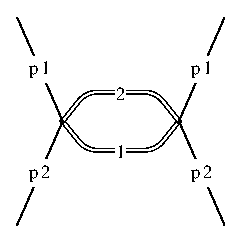
\includegraphics[scale=0.8]{top-type.1.eps}\hspace*{1.5pc}
  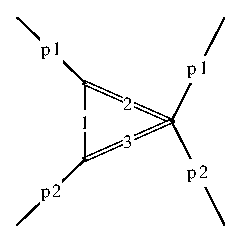
\includegraphics[scale=0.8]{top-type.2.eps}\hspace*{1.5pc}
  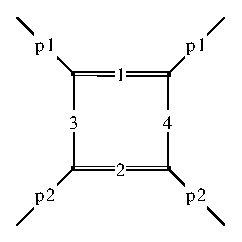
\includegraphics[scale=0.8]{top-type.3.eps}\hspace*{1.5pc}
  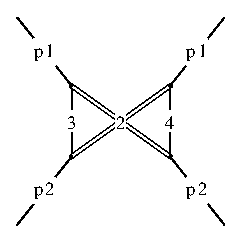
\includegraphics[scale=0.8]{top-type.4.eps}
  \caption{%
    Sample one-loop topologies appearing after asymptotic expansion at
    LO, NLO and NNLO (the last two).  The first graph is an example of a
    linearly independent, but incomplete topology.  The second topology
    is a linearly independent and complete.  The last two topologies,
    one planar, one non-planar, are linearly dependent and complete.
    Plain black lines are massless, the double lines carry the Higgs
    mass.}
  \label{fig::top-type}
\end{figure}

\begin{figure}
  \centering
  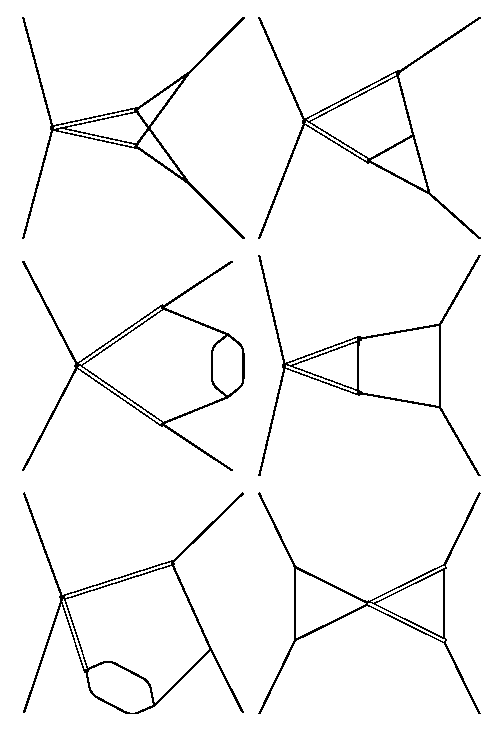
\includegraphics[scale=0.6]{NNLOgv22.gtops.eps}\hspace*{3.5pc}
  \includegraphics[scale=0.6]{NNLOgv22.ptops.eps}
  \caption{%
    The left hand side shows the set of diagram topologies, the right
    hand side the set of reduction topologies.  Their order is chosen by
    {\tt TopoID} in a fixed way, numbers in braces denote the presence
    of irreducible numerators.  The last topology in both sets is an
    example of a factorizing topology.  Note the modification of
    self-energy insertions from the left to the right side, propagators
    carrying the same momentum are identified.  Furthermore, there is a
    non-trivial mapping from the second and fourth diagram topology to
    the fourth reduction topology which cannot be deduced from the
    graphs alone.}
  \label{fig::tops-NNLOgv22}
\end{figure}













\section{Generalities}

\section{Applications}

% To 1-5-loop propagators

\subsection{Topology classification}

\subsubsection{Scheme A}

\subsubsection{Scheme B}

\subsection{\FORM code generation}

\subsection{Master integrals}

\subsubsection{Simple identification}

\subsubsection{Additional relations}

\subsection{``Super''-topologies}

\section{Provided functions}

\section{Interfaces}

\subsection{{\tt QGRAF}}

\subsection{{\tt MATAD}}

\subsection{{\tt FIRE}, {\tt asy.m}}

\subsection{{\tt feynMF}}




















\end{document}
